% New analysis update started from zero on 2026-08-13.
% Scientific sources:
%   ../docs/progress.md
%   ../XGBoost/docs/knowledge/post_20260805_ml_delta_for_slides.md
%   ../Analysis_CODES/docs/slides_20260813_codes_delta.md
\documentclass[11pt,aspectratio=169]{beamer}

\usetheme{Madrid}
\usecolortheme{default}
\setbeamertemplate{navigation symbols}{}
\setbeamertemplate{footline}[frame number]

\usepackage{booktabs}
\usepackage{graphicx}
\usepackage{tikz}
\usetikzlibrary{arrows.meta,positioning}
\input{beamer_setup.tex}

% Optional fast single-frame build, e.g.:
%   bash fastcompile_frame.sh p2
\ifdefined\onlyframes
  \expandafter\includeonlyframes\expandafter{\onlyframes}
\fi

\definecolor{positive}{HTML}{0173B2}
\definecolor{negative}{HTML}{DE8F05}
\definecolor{emphasis}{HTML}{027A5A}
\definecolor{neutral}{HTML}{666666}
\definecolor{panelbg}{HTML}{F4F6F8}
\setbeamercolor{structure}{fg=positive}
\setbeamercolor{block title}{fg=white,bg=positive}
\setbeamercolor{block body}{fg=black,bg=positive!8}
\setbeamercolor{block title alerted}{fg=white,bg=negative}
\setbeamercolor{block body alerted}{fg=black,bg=negative!10}
\setbeamercolor{block title example}{fg=white,bg=emphasis}
\setbeamercolor{block body example}{fg=black,bg=emphasis!8}
\newcommand{\pos}[1]{\textcolor{positive}{#1}}
\newcommand{\con}[1]{\textcolor{negative}{#1}}
\newcommand{\HL}[1]{\textcolor{emphasis}{#1}}
\newcommand{\muted}[1]{\textcolor{neutral}{#1}}

\title[X(3872) Analysis Update]{X(3872) Analysis Update}
\subtitle{new findings in reweighting and ML}
\author{%
  Henrique Legoinha, \underline{Lekai Yao}, Nuno Leonardo, Zhen Hu\\[0.45em]
  2026.8.13%
}
\institute{}
\date{%
  \includegraphics[height=1.653cm]{figures/symbols/CERN.png}\hspace{0.30cm}%
  \includegraphics[height=1.653cm]{figures/symbols/CMS.png}\hspace{0.30cm}%
  \includegraphics[height=1.653cm]{figures/symbols/LIP.png}\hspace{0.30cm}%
  \includegraphics[height=1.653cm]{figures/symbols/LU.png}\hspace{0.30cm}%
  \includegraphics[height=1.653cm]{figures/symbols/THU.png}%
}

\begin{document}

\begin{frame}[plain,label=p1]
  \titlepage
\end{frame}

\begin{frame}[label=p2]{Recap: two routes we tried}
  \vspace{0.25em}
  \begin{columns}[T]
    \begin{column}{0.48\textwidth}
      \centering
      {\large\bfseries \psiP ppRef/PbPb weight $\rightarrow$ X}\par
      \vspace{0.55em}
      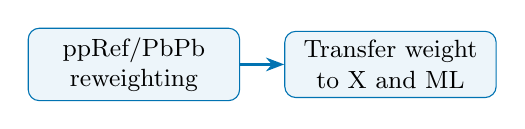
\begin{tikzpicture}[
        node distance=0.56cm,
        routebox/.style={draw=positive,rounded corners,fill=positive!7,
          minimum height=0.72cm,text width=2.45cm,align=center,font=\small},
        arr/.style={-{Stealth},thick,positive}
      ]
        \node[routebox] (a) {ppRef/PbPb \psiP\\reweighting};
        \node[routebox,right=of a] (b) {Transfer weight\\to X and ML};
        \draw[arr] (a) -- (b);
      \end{tikzpicture}

      \vspace{0.75em}
      \raggedright
      \textbf{What stopped this route}
      \begin{itemize}
        \setlength{\itemsep}{0.35em}
        \item \psiP and X MC have different variable distributions.
        \item In PbPb, no sufficiently significant \psiP peak was available for reweighting.
      \end{itemize}
    \end{column}

    \begin{column}{0.48\textwidth}
      \centering
      {\large\bfseries X ppRef weight $\rightarrow$ PbPb}\par
      \vspace{0.55em}
      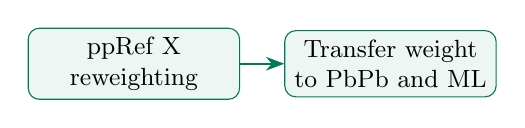
\begin{tikzpicture}[
        node distance=0.56cm,
        routebox/.style={draw=emphasis,rounded corners,fill=emphasis!7,
          minimum height=0.72cm,text width=2.45cm,align=center,font=\small},
        arr/.style={-{Stealth},thick,emphasis}
      ]
        \node[routebox] (a) {ppRef X\\reweighting};
        \node[routebox,right=of a] (b) {Transfer weight\\to PbPb and ML};
        \draw[arr] (a) -- (b);
      \end{tikzpicture}

      \vspace{0.75em}
      \raggedright
      \textbf{What stopped this route}
      \begin{itemize}
        \setlength{\itemsep}{0.35em}
        \item X ppRef and PbPb MC showed different input distributions.
        \item No visible X peak remained after the transfer and ML selection.
      \end{itemize}
    \end{column}
  \end{columns}

\end{frame}

\begin{frame}[label=p3]{How the present strategy emerged}
  \vfill
  \centering
  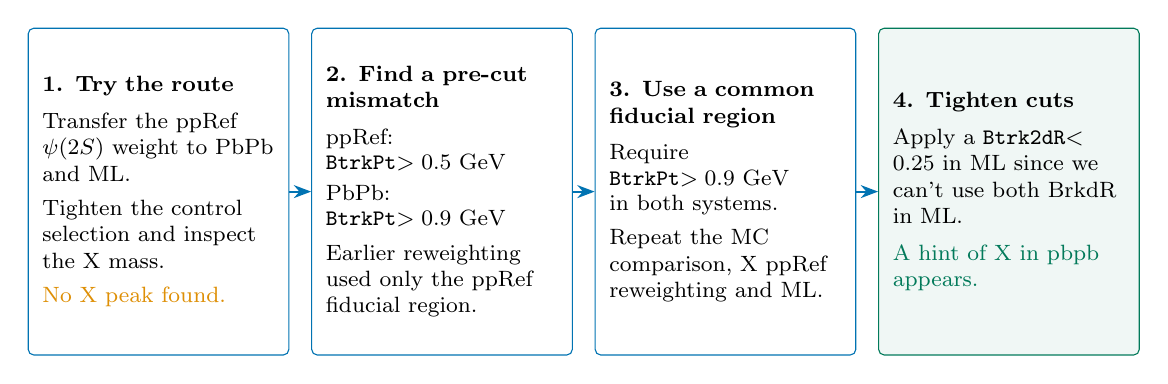
\begin{tikzpicture}[
    x=1cm,y=1cm,
    stage/.style={
      draw=positive,
      rounded corners=2pt,
      fill=white,
      minimum height=4.15cm,
      text width=2.95cm,
      align=left,
      inner sep=0.18cm,
      font=\footnotesize,
      execute at begin node={\hyphenpenalty=10000\exhyphenpenalty=10000}
    },
    arr/.style={-{Stealth[length=2.2mm]},thick,positive}
  ]
    \node[stage] (s1) at (0,0) {\textbf{1. Try the \psiP route}\\[0.45em]
      Transfer the ppRef $\psi(2S)$ weight to PbPb and ML.\\[0.35em]
      Tighten the control selection and inspect the X mass.\\[0.35em]
      \con{No X peak found.}};

    \node[stage] (s2) at (3.60,0) {\textbf{2. Find a pre-cut mismatch}\\[0.45em]
      ppRef:\\[-0.05em]
      \texttt{BtrkPt}$>0.5$ GeV\\[0.2em]
      PbPb:\\[-0.05em]
      \texttt{BtrkPt}$>0.9$ GeV\\[0.35em]
      Earlier reweighting used only the ppRef fiducial region.};

    \node[stage] (s3) at (7.20,0) {\textbf{3. Use a common fiducial region}\\[0.45em]
      Require\\[-0.05em]
      \texttt{BtrkPt}$>0.9$ GeV\\[-0.05em]
      in both systems.\\[0.35em]
      Repeat the MC comparison, X ppRef reweighting and ML.};

    \node[stage,draw=emphasis,fill=emphasis!6] (s4) at (10.80,0) {\textbf{4. Tighten cuts}\\[0.45em]
      Apply a \texttt{Btrk2dR}$<0.25$ in ML since we can't use both BrkdR in ML.\\[0.45em]
      \HL{A hint of X in pbpb appears.}};

    \draw[arr] (s1.east) -- (s2.west);
    \draw[arr] (s2.east) -- (s3.west);
    \draw[arr] (s3.east) -- (s4.west);
  \end{tikzpicture}
  \vfill
\end{frame}

\begin{frame}[label=p4]{$\psi(2S)$ ppRef weight $\rightarrow$ PbPb workflow}
  \centering
  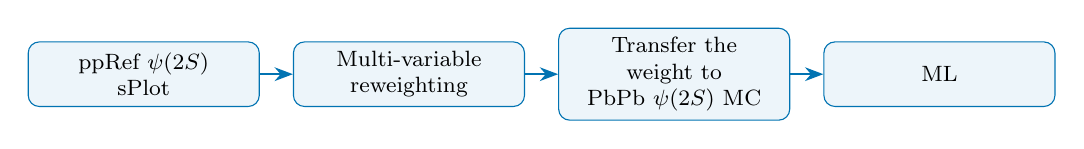
\begin{tikzpicture}[
    node distance=0.42cm,
    box/.style={draw=positive,rounded corners,fill=positive!7,
      text width=2.70cm,minimum height=0.82cm,align=center,font=\footnotesize},
    arr/.style={-{Stealth},thick,positive}
  ]
    \node[box] (a) {ppRef $\psi(2S)$\\sPlot};
    \node[box,right=of a] (b) {Multi-variable\\reweighting};
    \node[box,right=of b] (c) {Transfer the weight to\\PbPb $\psi(2S)$ MC};
    \node[box,right=of c] (d) {ML};
    \draw[arr] (a)--(b); \draw[arr] (b)--(c); \draw[arr] (c)--(d);
  \end{tikzpicture}

  \vspace{0.55em}
  \begin{block}{Common reweighting setting}
    \small
    \centering
    Variables: [\texttt{Bcos\_dtheta}, \texttt{Btktkpt}, \texttt{Bchi2Prob},
    \texttt{Btrk2Pt}, \texttt{Btrk1Pt}]\\[0.25em]
    $10<\texttt{Bpt}<50$ GeV, $|\texttt{By}|<1.6$, $\texttt{BQvalue}<0.15$,
    $2<\texttt{Btktkpt}<10$ GeV, $\texttt{Btrk1dR}<0.5$
  \end{block}

  \begin{columns}[T]
    \begin{column}{0.48\textwidth}
      \centering
      \textbf{R5range2}\\[0.25em]
      {\normalsize\texttt{BtrkPt}$>0.5$ GeV}
    \end{column}
    \begin{column}{0.48\textwidth}
      \centering
      \textbf{R5range3}\\[0.25em]
      {\normalsize\texttt{BtrkPt}$>1.0$ GeV}
    \end{column}
  \end{columns}
  \vfill
  \centering\small
  Flat-tree pre-cuts: ppRef \texttt{BtrkPt}$>0.5$ GeV; PbPb \texttt{BtrkPt}$>0.9$ GeV.
\end{frame}

\begin{frame}[label=p5]{Aligning the \texttt{BtrkPt} pre-cut aligns the MC domains}
  \begin{columns}[T]
    \begin{column}{0.49\textwidth}
      \centering
      \textbf{R5range2: effective pre-cuts differ}\\[-0.1em]
      \includegraphics[width=0.70\linewidth]{../XGBoost/output/reweighting/X_pp24_psi2s_R5range2_rw_v1/ppref_pbpb24_psi2s_mc_comparison_v1/pb24_fid6/variables/Btrk1Pt_ppref_vs_pbpb24_psi2s_unweighted.pdf}
      \vspace{-0.45em}
      \small\mbox{KS-like distance $=0.1876$}\\
      R8 mean $=0.10709$
    \end{column}
    \begin{column}{0.49\textwidth}
      \centering
      \textbf{R5range3: common pre-cut}\\[-0.1em]
      \includegraphics[width=0.70\linewidth]{../XGBoost/output/reweighting/X_pp24_psi2s_R5range3_rw_v1/ppref_pbpb24_psi2s_mc_comparison_v1/pb24_fid8/variables/Btrk1Pt_ppref_vs_pbpb24_psi2s_unweighted.pdf}
      \vspace{-0.45em}
      \small\mbox{KS-like distance $=0.0172$}\\
      R8 mean $=0.01721$
    \end{column}
  \end{columns}
  \vfill
  \begin{beamercolorbox}[wd=0.92\textwidth,sep=0.34em,center,rounded=true]{block body example}
    With the same \texttt{BtrkPt} pre-cut, ppRef and PbPb $\psi(2S)$ MC are very close.
  \end{beamercolorbox}
\end{frame}

\begin{frame}[label=p6]{ML settings based on the same reweighting R5range3}
  \footnotesize
  \begin{block}{Weighted ML baseline}
    $10<\texttt{Bpt}<50$ GeV, $|\texttt{By}|<1.6$, $\texttt{BQvalue}<0.15$,
    $\texttt{BtrkPt}>1.0$ GeV, $2<\texttt{Btktkpt}<10$ GeV,
    $\texttt{Btrk1dR}<0.5$\\[0.25em]
    Variables: [\texttt{Bchi2Prob}, \texttt{Btrk1dR}, \texttt{BtrkPtimb},
    \texttt{Btrk1Pt}, \texttt{Btrk2Pt}, \texttt{BtktkvProb},
    \texttt{Bcos\_dtheta}, \texttt{Btktkpt}]\\[0.2em]
    {\scriptsize Baseline tag: \texttt{X\_pb24\_v7\_fid8\_8v2\_rwpsi2sr5range3v1\_xgb\_v1}}
  \end{block}

  \vspace{-0.2em}
  \renewcommand{\arraystretch}{1.14}
  \begin{tabular}{p{6.25cm}p{7.05cm}}
    \toprule
    Train tag & Difference from the weighted 8-variable baseline \\
    \midrule
    \shortstack[l]{\scriptsize\texttt{X\_pb24\_v7\_fid8\_8v2\_}\\[-0.1em]
     \scriptsize\texttt{rwpsi2srawv1\_xgb\_v1}}
      & Use raw $\psi(2S)$ PbPb MC without weight \\
    \addlinespace[0.20em]
    \shortstack[l]{\scriptsize\texttt{X\_pb24\_v7\_fid8\_6v5\_}\\[-0.1em]
     \scriptsize\texttt{rwpsi2sr5range3v1\_xgb\_v1}}
      & Remove \texttt{BtrkPtimb} and \texttt{BtktkvProb} \\
    \addlinespace[0.20em]
    \shortstack[l]{\scriptsize\texttt{X\_pb24\_v7\_fid8\_7v2\_}\\[-0.1em]
     \scriptsize\texttt{rwpsi2sr5range3v1\_xgb\_v1}}
      & Add \texttt{Btrk2dR}; remove \texttt{Btrk2Pt} and \texttt{BtktkvProb} \\
    \addlinespace[0.20em]
    \shortstack[l]{\scriptsize\texttt{X\_pb24\_v8\_fid9\_8v2\_}\\[-0.1em]
     \scriptsize\texttt{rwpsi2sr5range3dr045v1\_xgb\_v1}}
      & Add \texttt{Btrk2dR}$<0.45$ selection \\
    \bottomrule
  \end{tabular}
\end{frame}

\begin{frame}[label=p7]{The $\psi(2S)$ control improves, but X remains absent}
  \centering
  \small Weighted ML baseline; score cuts are defined by weighted $\psi(2S)$ efficiency.
  \vspace{0.35em}
  \begin{columns}[T]
    \begin{column}{0.49\textwidth}
      \centering
      \textbf{Loose ML selection: 80\% efficiency}\\[0.2em]
      \includegraphics[width=0.65\linewidth,trim=0 0 0 0.58in,clip]{../XGBoost/output/selected/X_pb24_v7_fid8_8v2_rwpsi2sr5range3v1_xgb_v1/cut_scan/weighted_signal_efficiency/DATA_pb24_fid8_eff080.pdf}
    \end{column}
    \begin{column}{0.49\textwidth}
      \centering
      \textbf{Tight ML selection: 20\% efficiency}\\[0.2em]
      \includegraphics[width=0.65\linewidth,trim=0 0 0 0.58in,clip]{../XGBoost/output/selected/X_pb24_v7_fid8_8v2_rwpsi2sr5range3v1_xgb_v1/cut_scan/weighted_signal_efficiency/DATA_pb24_fid8_eff020.pdf}
    \end{column}
  \end{columns}
  \vfill
  \begin{beamercolorbox}[wd=0.93\textwidth,sep=0.34em,center,rounded=true]{block body alerted}
    Across the five ML settings, tighter selections enhance the $\psi(2S)$ peak,\\
    but no clear narrow X peak is visible.
  \end{beamercolorbox}
\end{frame}

\begin{frame}[label=p8]{Why return to X ppRef weight $\rightarrow$ PbPb?}
  \begin{columns}[T]
    \begin{column}{0.46\textwidth}
      \begin{block}{What the $\psi(2S)$ route established}
        \begin{itemize}
          \item Common \texttt{BtrkPt} pre-cuts bring ppRef and PbPb $\psi(2S)$ MC close.
          \item ML selections produce a stronger $\psi(2S)$ control peak.
        \end{itemize}
      \end{block}
    \end{column}
    \begin{column}{0.46\textwidth}
      \begin{alertblock}{What it did not deliver}
        \begin{itemize}
          \item None of the five ML settings produced a clear narrow X peak.
          \item The optimization of ML performance was not studied in detail.
        \end{itemize}
      \end{alertblock}
    \end{column}
  \end{columns}
  \vspace{0.65em}
  \centering
  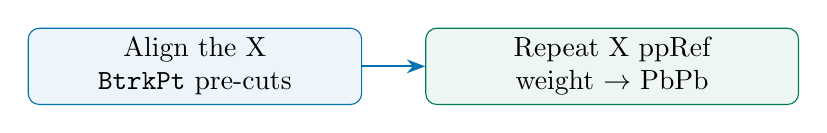
\begin{tikzpicture}[node distance=0.8cm]
    \node[draw=positive,rounded corners,fill=positive!7,text width=4.0cm,
      align=center,minimum height=0.95cm] (a) {Align the X \texttt{BtrkPt} pre-cuts};
    \node[draw=emphasis,rounded corners,fill=emphasis!7,text width=4.5cm,
      align=center,minimum height=0.95cm,right=of a] (b) {Repeat X ppRef weight $\rightarrow$ PbPb};
    \draw[-{Stealth},thick,positive] (a)--(b);
  \end{tikzpicture}
\end{frame}

\begin{frame}[label=p9]{Aligning the \texttt{BtrkPt} pre-cut aligns the X MC domains}
  \begin{columns}[T]
    \begin{column}{0.49\textwidth}
      \centering
      \textbf{Original: different pre-cuts}\\[-0.1em]
      \includegraphics[width=0.70\linewidth]{../XGBoost/output/reweighting/X_pp24_xsplot_R6range5_rw_v1/ppref_pbpb_mc_comparison_v1/common_fiducial_baseline/variables/Btrk2Pt_ppref_vs_pbpb_unweighted.pdf}
      \vspace{-0.45em}
      \small\mbox{KS-like distance $=0.1626$}\\
      R8 mean $=0.09413$
    \end{column}
    \begin{column}{0.49\textwidth}
      \centering
      \textbf{Same pre-cut: \texttt{BtrkPt}$>0.9$ GeV}\\[-0.1em]
      \includegraphics[width=0.70\linewidth]{../XGBoost/output/reweighting/X_pp24_xsplot_R6range5_rw_v1/ppref_pbpb_mc_comparison_v1/common_fiducial_in_reweight_support/variables/Btrk2Pt_ppref_vs_pbpb_unweighted.pdf}
      \vspace{-0.45em}
      \small\mbox{KS-like distance $=0.0049$}\\
      R8 mean $=0.01307$
    \end{column}
  \end{columns}
  \vfill
  \begin{beamercolorbox}[wd=0.92\textwidth,sep=0.34em,center,rounded=true]{block body example}
    With the same \texttt{BtrkPt} pre-cut, ppRef and PbPb X MC are very close.
  \end{beamercolorbox}
\end{frame}

\begin{frame}[label=p10]{X ppRef weight $\rightarrow$ PbPb: workflow}
  \centering
  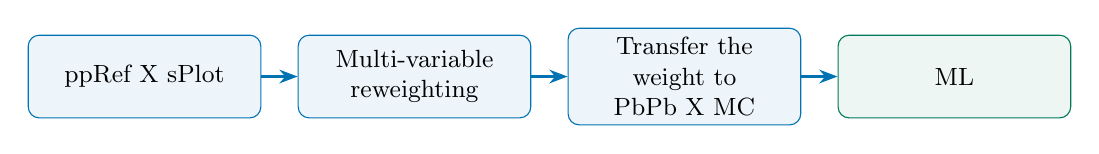
\begin{tikzpicture}[
    node distance=0.46cm,
    box/.style={draw=positive,rounded corners,fill=positive!7,text width=2.72cm,
      minimum height=1.05cm,align=center,font=\small},
    arr/.style={-{Stealth},thick,positive}
  ]
    \node[box] (a) {ppRef X sPlot};
    \node[box,right=of a] (b) {Multi-variable\\reweighting};
    \node[box,right=of b] (c) {Transfer the weight to\\PbPb X MC};
    \node[box,right=of c,draw=emphasis,fill=emphasis!7] (d) {ML};
    \draw[arr] (a)--(b);
    \draw[arr] (b)--(c);
    \draw[arr] (c)--(d);
  \end{tikzpicture}

  \vspace{0.85em}
  \begin{columns}[T]
    \begin{column}{0.47\textwidth}
      \begin{block}{What changes were tried}
        \begin{itemize}
          \setlength{\itemsep}{0.40em}
          \item Same pre-cut
          \item Different reweighting variables \& fiducial regions
          \item Different ML variables \& fiducial regions
        \end{itemize}
      \end{block}
    \end{column}
    \begin{column}{0.47\textwidth}
      \begin{exampleblock}{What improved}
        \begin{itemize}
          \setlength{\itemsep}{0.40em}
          \item ppRef/PbPb MC agreement in the same fiducial region
          \item ML-to-fit workflow
          \item A hint of X in PbPb
        \end{itemize}
      \end{exampleblock}
    \end{column}
  \end{columns}
\end{frame}

\begin{frame}[label=p11]{Three X ppRef reweighting settings and ML follow-ups}
  \footnotesize
  \centering
  \textbf{Common variables:}
  [\texttt{Bcos\_dtheta}, \texttt{Btktkpt}, \texttt{Bchi2Prob},
  \texttt{Btrk1Pt}, \texttt{Btrk1dR}]\\[0.12em]
  \textbf{Common region:}
  $10<\texttt{Bpt}<50$ GeV, $|\texttt{By}|<1.6$, $\texttt{BQvalue}<0.15$,
  $2<\texttt{Btktkpt}<8$ GeV, $\texttt{BtrkPt}>0.9$ GeV

  \vspace{0.45em}
  \scriptsize
  \renewcommand{\arraystretch}{1.14}
  \begin{tabular}{p{1.95cm}p{4.15cm}p{6.95cm}}
    \toprule
    Setting & BDT reweighting variables and region & ML follow-up \\
    \midrule
    \textbf{R5v2range3} &
      \begin{tabular}[t]{@{}l@{}}Variables: common set\\Region: \texttt{Btrk1Pt}$\leq4.5$ GeV\end{tabular} &
      No ML follow-up \\
    \textbf{R6range3} &
      \begin{tabular}[t]{@{}l@{}}Variables: common $+$ \texttt{Btrk2Pt}\\Region: \texttt{BtrkPt}$\leq4.5$ GeV\end{tabular} &
      \begin{tabular}[t]{@{}p{6.50cm}@{}}
        8v2: [\texttt{Bchi2Prob}, \texttt{Btrk1dR}, \texttt{BtrkPtimb},
        \texttt{Btrk1Pt}, \texttt{Btrk2Pt}, \texttt{BtktkvProb},
        \texttt{Bcos\_dtheta}, \texttt{Btktkpt}]\\
        6v5: [\texttt{Btrk1dR}, \texttt{Btktkpt}, \texttt{Btrk1Pt},
        \texttt{Bchi2Prob}, \texttt{Bcos\_dtheta}, \texttt{Btrk2Pt}]\\
        6v5 regions: \texttt{Btrk2dR}$<0.45$ and $<0.25$
      \end{tabular} \\
    \textbf{R6v2range3} &
      \begin{tabular}[t]{@{}l@{}}Variables: common $+$ \texttt{Btrk2dR}\\Region: \texttt{Btrk2dR}$<0.5$\end{tabular} &
      \begin{tabular}[t]{@{}p{6.50cm}@{}}
        8v2: same variable set as above\\
        9v2: [\texttt{Btrk1dR}, \texttt{Btrk2dR}, \texttt{Btktkpt},
        \texttt{Btrk1Pt}, \texttt{Btrk2Pt}, \texttt{Bchi2Prob},
        \texttt{Bcos\_dtheta}, \texttt{BtrkPtimb}, \texttt{BtktkvProb}]
      \end{tabular} \\
    \bottomrule
  \end{tabular}

  \vspace{0.25em}
  \centering
  \footnotesize
  Different reweighting variables were tested to find the most suitable variable set.
\end{frame}

\begin{frame}[label=p12]{\texttt{Btrk1dR} sWeighted-data closure}
  \begin{columns}[T]
    \begin{column}{0.325\textwidth}
      \centering
      \textbf{R5v2range3}\par\vspace{-0.15em}
      \includegraphics[width=\linewidth]{../XGBoost/output/reweighting/X_pp24_xsplot_R5v2range3_rw_v1/transfer_closure_x_splot_v1/variables/Btrk1dR_transfer_closure.pdf}
      \vspace{-0.45em}
      \small KS-like distance\\
      \texttt{Btrk1dR}: $0.0856\rightarrow0.0646$\\
      Mean: $0.1403\rightarrow0.0410$
    \end{column}
    \begin{column}{0.325\textwidth}
      \centering
      \textbf{R6range3}\par\vspace{-0.15em}
      \includegraphics[width=\linewidth]{../XGBoost/output/reweighting/X_pp24_xsplot_R6range3_rw_v1/transfer_closure_x_splot_v1/variables/Btrk1dR_transfer_closure.pdf}
      \vspace{-0.45em}
      \small KS-like distance\\
      \texttt{Btrk1dR}: $0.0860\rightarrow0.0612$\\
      Mean: $0.1350\rightarrow0.0395$
    \end{column}
    \begin{column}{0.325\textwidth}
      \centering
      \textbf{R6v2range3}\par\vspace{-0.15em}
      \includegraphics[width=\linewidth]{../XGBoost/output/reweighting/X_pp24_xsplot_R6v2range3_rw_v1/transfer_closure_x_splot_v1/variables/Btrk1dR_transfer_closure.pdf}
      \vspace{-0.45em}
      \small KS-like distance\\
      \texttt{Btrk1dR}: $0.0879\rightarrow0.0901$\\
      Mean: $0.1423\rightarrow0.0673$
    \end{column}
  \end{columns}
\end{frame}

\begin{frame}[label=p13]{A pronounced peak-like feature at xeff 20\%}
  \begin{columns}[T]
    \begin{column}{0.63\textwidth}
      \centering
      \includegraphics[height=0.72\textheight,trim=0 0 0 35,clip]
      {../XGBoost/output/selected/X_pb24_v12_fid13_6v5_rwr6range3dr025v1_xgb_v1/cut_scan/weighted_signal_efficiency/DATA_pb24_fid13_eff020.pdf}
    \end{column}
    \begin{column}{0.34\textwidth}
      \begin{block}{Setting}
        \footnotesize
        \begin{itemize}
          \setlength{\itemsep}{0.25em}
          \item R6range3 weight
          \item ML variables: [\texttt{Btrk1dR}, \texttt{Btktkpt},
            \texttt{Btrk1Pt}, \texttt{Bchi2Prob},
            \texttt{Bcos\_dtheta}, \texttt{Btrk2Pt}]
          \item ML fiducial region: \texttt{Btrk2dR}$<0.25$
          \item Weighted signal efficiency: 20\%
        \end{itemize}
      \end{block}
      \vspace{0.25em}
      \small
      Unlike the previous ML settings, a pronounced local feature appears near the X mass.
    \end{column}
  \end{columns}

  \vfill
  \centering\HL{Mass-spectrum observation before a dedicated fit interpretation.}
\end{frame}

\begin{frame}[label=p14]{Scanning the \texttt{Btrk2dR} region in reweighting and ML}
  \footnotesize
  \begin{block}{Common setting}
    \centering
    Reweighting variables: [\texttt{Bcos\_dtheta}, \texttt{Btktkpt},
    \texttt{Bchi2Prob}, \texttt{Btrk2Pt}, \texttt{Btrk1Pt}, \texttt{Btrk1dR}]\\[0.18em]
    ML variables: [\texttt{Btrk1dR}, \texttt{Btktkpt}, \texttt{Btrk1Pt},
    \texttt{Bchi2Prob}, \texttt{Bcos\_dtheta}, \texttt{Btrk2Pt}]
  \end{block}

  \vspace{0.25em}
  \centering
  \renewcommand{\arraystretch}{1.24}
  \begin{tabular}{lccc}
    \toprule
    Reweighting setting & Reweighting fiducial region & ML setting & ML fiducial region \\
    \midrule
    \textbf{R6range4} & \texttt{Btrk2dR}$<0.45$ & 6v5 with R6range4 weight & \texttt{Btrk2dR}$<0.45$ \\
    \textbf{R6range5} & \texttt{Btrk2dR}$<0.40$ & 6v5 with R6range5 weight & \texttt{Btrk2dR}$<0.40$ \\
    \textbf{R6range6} & \texttt{Btrk2dR}$<0.35$ & 6v5 with R6range6 weight & \texttt{Btrk2dR}$<0.35$ \\
    \textbf{R6range7} & \texttt{Btrk2dR}$<0.30$ & 6v5 with R6range7 weight & \texttt{Btrk2dR}$<0.30$ \\
    \textbf{R6range8} & \texttt{Btrk2dR}$<0.25$ & 6v5 with R6range8 weight & \texttt{Btrk2dR}$<0.25$ \\
    \bottomrule
  \end{tabular}

  \vfill
  \centering
  For each setting, reweighting and ML use the same \texttt{Btrk2dR} fiducial region.
\end{frame}

\begingroup
\newcommand{\fitcell}[3]{\shortstack{$#1\sigma\,/$\\$#2\pm#3$}}
\newcommand{\boundcell}[3]{\shortstack{$#1\sigma\,/$\con{[B]}\\$#2\pm#3$}}
\newcommand{\badcell}[3]{\shortstack{$#1\sigma\,/$\textcolor{neutral}{[F]}\\$#2\pm#3$}}
\begin{frame}[label=p15]{Nominal-fit scan across the five settings}
  \scriptsize
  \centering
  \textbf{DATA-only nominal fit:}
  extended unbinned fit in $3.80<\texttt{Bmass}<3.94$ GeV;
  single Gaussian, $3.86<\mu<3.88$ GeV, $0.1<\sigma<10$ MeV;
  Chebyshev-2 background.\\[0.12em]
  \textbf{xeff scan:} strict \texttt{Prediction}$>$threshold at weighted
  signal efficiency $=10,15,20,25,30,35,40\%$.

  \vspace{0.35em}
  \centering
  \textbf{Each cell: local significance $\sigma$ / fitted yield $\pm$ stat.}\par\vspace{0.20em}
  \renewcommand{\arraystretch}{1.24}
  \setlength{\tabcolsep}{4.0pt}
  \begin{tabular}{lccccccc}
    \toprule
    Setting $\backslash$ xeff & 10\% & 15\% & 20\% & 25\% & 30\% & 35\% & 40\% \\
    \midrule
    \textbf{R6range4} &
      \fitcell{2.11}{33.4}{16.1} & \fitcell{1.42}{36.4}{25.2} & \boundcell{0.00}{0.1}{239.7} &
      \fitcell{0.55}{15.7}{34.2} & \boundcell{1.56}{56.6}{44.5} & \fitcell{1.39}{65.5}{51.9} & \fitcell{1.08}{61.0}{62.9} \\
    \midrule
    \textbf{R6range5} &
      \boundcell{1.92}{29.1}{15.0} & \fitcell{2.09}{42.0}{30.4} & \fitcell{1.37}{44.1}{46.4} &
      \fitcell{1.15}{31.9}{33.0} & \boundcell{0.93}{23.1}{28.4} & \fitcell{1.57}{68.7}{48.2} & \fitcell{1.55}{80.6}{58.6} \\
    \midrule
    \textbf{R6range6} &
      \fitcell{2.00}{27.5}{13.5} & \boundcell{1.82}{40.6}{22.2} & \boundcell{1.13}{35.0}{30.7} &
      \fitcell{0.76}{29.6}{36.7} & \boundcell{1.28}{64.7}{51.3} & \fitcell{1.55}{55.2}{42.6} & \fitcell{1.33}{52.7}{53.2} \\
    \midrule
    \textbf{R6range7} &
      \boundcell{2.75}{33.3}{11.8} & \fitcell{2.09}{16.6}{10.7} & \boundcell{1.57}{40.4}{25.6} &
      \boundcell{1.01}{32.6}{32.1} & \boundcell{0.74}{30.3}{40.6} & \fitcell{2.02}{41.3}{24.6} & \badcell{0.04}{2.7}{942.7} \\
    \midrule
    \textbf{R6range8} &
      \boundcell{1.99}{19.8}{9.6} & \fitcell{2.07}{12.2}{7.5} & \boundcell{1.60}{32.2}{19.9} &
      \fitcell{1.81}{27.0}{18.1} & \fitcell{1.45}{32.3}{28.6} & \fitcell{0.36}{13.6}{37.4} & \boundcell{0.00}{0.0}{48.5} \\
    \bottomrule
  \end{tabular}

  \vspace{0.35em}
  \centering
  \con{[B]} parameter boundary reported
  \qquad
  \textcolor{neutral}{[F]} fit status/covQual $\neq0/3$
\end{frame}
\endgroup

\begin{frame}[label=p16]{R6range7 nominal fits at xeff 10\% and 15\%}
  \begin{columns}[T,onlytextwidth]
    \begin{column}{0.49\textwidth}
      \centering
      {\large\bfseries xeff 10\%}\par
      \vspace{0.15em}
      \includegraphics[height=0.55\textheight]{../Analysis_CODES/fitER/results/H020_nominal_fit_batch/X_pb24_v16_fid17_6v5_rwr6range7v1_xgb_v1/data_only_nominal_v1/xeff10/data_fit.pdf}

      \vspace{0.25em}
      \small
      Local significance: $2.745\sigma$\\[0.12em]
      Yield: $33.26\pm11.80$ (stat.)\\[0.12em]
      Gaussian width: $10.000$ MeV \con{[boundary]}
    \end{column}
    \begin{column}{0.49\textwidth}
      \centering
      {\large\bfseries xeff 15\%}\par
      \vspace{0.15em}
      \includegraphics[height=0.55\textheight]{../Analysis_CODES/fitER/results/H020_nominal_fit_batch/X_pb24_v16_fid17_6v5_rwr6range7v1_xgb_v1/data_only_nominal_v1/xeff15/data_fit.pdf}

      \vspace{0.25em}
      \small
      Local significance: $2.088\sigma$\\[0.12em]
      Yield: $16.55\pm10.66$ (stat.)\\[0.12em]
      Gaussian width: $3.079$ MeV
    \end{column}
  \end{columns}
\end{frame}

\begin{frame}[label=p17]{Fixing the ML \texttt{Btrk2dR} region while varying reweighting}
  \footnotesize
  \begin{block}{Common setting}
    \centering
    Reweighting variables: [\texttt{Bcos\_dtheta}, \texttt{Btktkpt},
    \texttt{Bchi2Prob}, \texttt{Btrk2Pt}, \texttt{Btrk1Pt}, \texttt{Btrk1dR}]\\[0.18em]
    ML variables: [\texttt{Btrk1dR}, \texttt{Btktkpt}, \texttt{Btrk1Pt},
    \texttt{Bchi2Prob}, \texttt{Bcos\_dtheta}, \texttt{Btrk2Pt}]
  \end{block}

  \vspace{0.25em}
  \centering
  \renewcommand{\arraystretch}{1.30}
  \begin{tabular}{lccc}
    \toprule
    Reweighting setting & Reweighting fiducial region & ML setting & ML fiducial region \\
    \midrule
    \textbf{R6range4} & \texttt{Btrk2dR}$<0.45$ & 6v5 with R6range4 weight & \texttt{Btrk2dR}$<0.25$ \\
    \textbf{R6range5} & \texttt{Btrk2dR}$<0.40$ & 6v5 with R6range5 weight & \texttt{Btrk2dR}$<0.25$ \\
    \textbf{R6range6} & \texttt{Btrk2dR}$<0.35$ & 6v5 with R6range6 weight & \texttt{Btrk2dR}$<0.25$ \\
    \textbf{R6range7} & \texttt{Btrk2dR}$<0.30$ & 6v5 with R6range7 weight & \texttt{Btrk2dR}$<0.25$ \\
    \bottomrule
  \end{tabular}

  \vfill
  \centering
  The ML fiducial region is fixed; only the transferred weight setting changes.
\end{frame}

\begingroup
\newcommand{\fitcell}[3]{\shortstack{$#1\sigma\,/$\\$#2\pm#3$}}
\newcommand{\boundcell}[3]{\shortstack{$#1\sigma\,/$\con{[B]}\\$#2\pm#3$}}
\newcommand{\badcell}[3]{\shortstack{$#1\sigma\,/$\textcolor{neutral}{[F]}\\$#2\pm#3$}}
\begin{frame}[label=p18]{Nominal-fit scan with a common ML \texttt{Btrk2dR} region}
  \scriptsize
  \centering
  \textbf{DATA-only nominal fit:}
  extended unbinned fit in $3.80<\texttt{Bmass}<3.94$ GeV;
  single Gaussian, $3.86<\mu<3.88$ GeV, $0.1<\sigma<10$ MeV;
  Chebyshev-2 background.\\[0.12em]
  \textbf{xeff scan:} strict \texttt{Prediction}$>$threshold at weighted
  signal efficiency $=10,15,20,25,30,35,40\%$.

  \vspace{0.42em}
  \textbf{Each cell: local significance $\sigma$ / fitted yield $\pm$ stat.}\par\vspace{0.24em}
  \renewcommand{\arraystretch}{1.34}
  \setlength{\tabcolsep}{4.5pt}
  \begin{tabular}{lccccccc}
    \toprule
    Setting $\backslash$ xeff & 10\% & 15\% & 20\% & 25\% & 30\% & 35\% & 40\% \\
    \midrule
    \textbf{R6range4} &
      \fitcell{1.67}{7.5}{5.7} & \fitcell{2.37}{27.9}{10.8} & \boundcell{2.50}{42.7}{17.3} &
      \fitcell{1.40}{22.6}{19.2} & \fitcell{2.14}{53.1}{40.8} & \fitcell{1.05}{19.8}{21.8} & \fitcell{2.65}{13.7}{6.5} \\
    \midrule
    \textbf{R6range5} &
      \fitcell{2.24}{18.7}{8.1} & \fitcell{2.24}{26.7}{11.8} & \fitcell{1.82}{30.5}{20.1} &
      \fitcell{2.33}{35.3}{18.2} & \fitcell{1.68}{33.8}{26.6} & \fitcell{1.27}{16.9}{17.3} & \fitcell{1.36}{25.3}{28.6} \\
    \midrule
    \textbf{R6range6} &
      \fitcell{2.15}{18.5}{10.1} & \fitcell{2.35}{29.4}{12.5} & \boundcell{2.48}{44.5}{17.9} &
      \fitcell{1.74}{26.3}{18.9} & \fitcell{1.66}{22.6}{18.4} & \fitcell{0.19}{5.8}{37.7} & \badcell{0.83}{14.5}{23.3} \\
    \midrule
    \textbf{R6range7} &
      \boundcell{2.16}{19.8}{8.9} & \boundcell{2.69}{36.3}{13.2} & \fitcell{1.30}{23.8}{18.1} &
      \fitcell{2.13}{36.3}{22.7} & \fitcell{1.46}{22.0}{17.5} & \fitcell{0.77}{15.6}{22.3} & \boundcell{1.50}{4.8}{3.7} \\
    \bottomrule
  \end{tabular}

  \vspace{0.42em}
  \con{[B]} parameter boundary reported
  \qquad
  \textcolor{neutral}{[F]} fit status/covQual $\neq0/3$
\end{frame}
\endgroup

\begin{frame}[label=p19]{Several best ML results}
  \begin{columns}[T,onlytextwidth]
    \begin{column}{0.32\textwidth}
      \centering
      \includegraphics[width=0.98\linewidth]{../Analysis_CODES/fitER/results/H020_nominal_fit_batch/X_pb24_v18_fid19_6v5_rwr6range4dr025v1_xgb_v1/data_only_nominal_v1/xeff15/data_fit.pdf}

      \vspace{0.20em}
      {\small\bfseries R6range4 $\cdot$ xeff 15\%}\par
      \vspace{0.20em}
      \footnotesize
      Local significance: $2.369\sigma$\\[0.10em]
      Yield: $27.89\pm10.82$ (stat.)\\[0.10em]
      Gaussian width: $9.982$ MeV
    \end{column}
    \begin{column}{0.32\textwidth}
      \centering
      \includegraphics[width=0.98\linewidth]{../Analysis_CODES/fitER/results/H020_nominal_fit_batch/X_pb24_v18_fid19_6v5_rwr6range5dr025v1_xgb_v1/data_only_nominal_v1/xeff25/data_fit.pdf}

      \vspace{0.20em}
      {\small\bfseries R6range5 $\cdot$ xeff 25\%}\par
      \vspace{0.20em}
      \footnotesize
      Local significance: $2.332\sigma$\\[0.10em]
      Yield: $35.28\pm18.21$ (stat.)\\[0.10em]
      Gaussian width: $6.237$ MeV
    \end{column}
    \begin{column}{0.32\textwidth}
      \centering
      \includegraphics[width=0.98\linewidth]{../Analysis_CODES/fitER/results/H020_nominal_fit_batch/X_pb24_v18_fid19_6v5_rwr6range6dr025v1_xgb_v1/data_only_nominal_v1/xeff15/data_fit.pdf}

      \vspace{0.20em}
      {\small\bfseries R6range6 $\cdot$ xeff 15\%}\par
      \vspace{0.20em}
      \footnotesize
      Local significance: $2.352\sigma$\\[0.10em]
      Yield: $29.37\pm12.48$ (stat.)\\[0.10em]
      Gaussian width: $9.988$ MeV
    \end{column}
  \end{columns}
\end{frame}

\begingroup
\newcommand{\fitcell}[3]{\shortstack{$#1\sigma\,/$\\$#2\pm#3$}}
\newcommand{\boundcell}[3]{\shortstack{$#1\sigma\,/$\con{[B]}\\$#2\pm#3$}}
\begin{frame}[label=p20]{Train-wide and application-tight test}
  \scriptsize
  \begin{block}{Common setting}
    \centering
    R6range5 weight; 6v5 ML variables;
    training region: \texttt{Btrk1dR}$<0.45$, \texttt{Btrk2dR}$<0.40$;\quad
    same XGBoost model
  \end{block}

  \centering
  \renewcommand{\arraystretch}{1.22}
  \begin{tabular}{lccc}
    \toprule
    Setting & Training region & Application/fit region & Train/test AUC \\
    \midrule
    \textbf{Baseline} & \texttt{Btrk2dR}$<0.40$ & \texttt{Btrk2dR}$<0.40$ & 0.88334 / 0.86113 \\
    \textbf{Train-wide/apply-tight} & \texttt{Btrk2dR}$<0.40$ & \texttt{Btrk2dR}$<0.25$ & same model \\
    \bottomrule
  \end{tabular}

  \vspace{0.30em}
  \con{Fit change for the new setting: Gaussian width range $[0.1,10]\rightarrow[2,8]$ MeV.}

  \vspace{0.28em}
  \textbf{Each cell: local significance $\sigma$ / fitted yield $\pm$ stat.}\par\vspace{0.18em}
  \renewcommand{\arraystretch}{1.27}
  \setlength{\tabcolsep}{4.3pt}
  \begin{tabular}{lccccccc}
    \toprule
    Setting $\backslash$ xeff & 10\% & 15\% & 20\% & 25\% & 30\% & 35\% & 40\% \\
    \midrule
    \textbf{Baseline} &
      \boundcell{1.92}{29.1}{15.0} & \fitcell{2.09}{42.0}{30.4} & \fitcell{1.37}{44.1}{46.4} &
      \fitcell{1.15}{31.9}{33.0} & \boundcell{0.93}{23.1}{28.4} & \fitcell{1.57}{68.7}{48.2} & \fitcell{1.55}{80.6}{58.6} \\
    \midrule
    \textbf{Apply-tight} &
      \fitcell{2.23}{14.5}{6.7} & \boundcell{2.09}{20.1}{10.0} & \boundcell{1.98}{28.5}{14.6} &
      \fitcell{2.23}{40.3}{22.1} & \boundcell{1.78}{41.4}{22.7} & \fitcell{1.76}{50.4}{30.6} & \fitcell{1.31}{26.0}{25.7} \\
    \bottomrule
  \end{tabular}

  \vfill
  \con{[B]} parameter boundary reported
  \qquad
  New setting: same training and model, tighter application/fit region.
\end{frame}

\begin{frame}[t,label=p21]{Narrower background mass region test}
  \scriptsize
  \centering
  \textbf{Common setting:} R6range5 weight; 6v5 ML variables; ML fiducial region:
  \texttt{Btrk1dR}$<0.45$, \texttt{Btrk2dR}$<0.25$

  \vspace{0.18em}
  \centering
  \renewcommand{\arraystretch}{1.14}
  \begin{tabular}{lccc}
    \toprule
    Setting & Background mass region [GeV] & XGBoost model & Train/test AUC \\
    \midrule
    \textbf{Baseline} & $[3.75,3.80]\cup[3.95,4.00]$ & baseline & 0.93936 / 0.92585 \\
    \textbf{Narrow background} & $[3.82,3.85]\cup[3.89,3.92]$ & retrained & 0.91844 / 0.89587 \\
    \bottomrule
  \end{tabular}

  \vspace{0.20em}
  \con{Fit change for the new setting: Gaussian width range $[0.1,10]\rightarrow[2,8]$ MeV.}

  \vspace{0.20em}
  \textbf{Each cell: local significance $\sigma$ / fitted yield $\pm$ stat.}\par\vspace{0.18em}
  \renewcommand{\arraystretch}{1.20}
  \setlength{\tabcolsep}{4.3pt}
  \begin{tabular}{lccccccc}
    \toprule
    Setting $\backslash$ xeff & 10\% & 15\% & 20\% & 25\% & 30\% & 35\% & 40\% \\
    \midrule
    \textbf{Baseline} &
      \fitcell{2.24}{18.7}{8.1} & \fitcell{2.24}{26.7}{11.8} & \fitcell{1.82}{30.5}{20.1} &
      \fitcell{2.33}{35.3}{18.2} & \fitcell{1.68}{33.8}{26.6} & \fitcell{1.27}{16.9}{17.3} & \fitcell{1.36}{25.3}{28.6} \\
    \midrule
    \textbf{Narrow background} &
      \boundcell{2.18}{5.9}{3.3} & \boundcell{3.08}{31.0}{10.5} & \boundcell{3.22}{45.0}{14.5} &
      \boundcell{3.25}{58.6}{18.7} & \boundcell{2.21}{49.7}{23.0} & \fitcell{1.93}{53.3}{27.8} & \fitcell{1.92}{62.7}{33.5} \\
    \bottomrule
  \end{tabular}

  \vfill
  \con{[B]} parameter boundary reported
  \qquad
  Background region and XGBoost model both change.
\end{frame}
\endgroup

\begin{frame}[label=p22]{Best ML result comparison}
  \begin{columns}[T,onlytextwidth]
    \begin{column}{0.49\textwidth}
      \centering
      \includegraphics[height=0.54\textheight]{../Analysis_CODES/fitER/results/H020_nominal_fit_batch/X_pb24_v18_fid19_6v5_rwr6range5dr025v1_xgb_v1/data_only_nominal_v1/xeff25/data_fit.pdf}

      \vspace{0.18em}
      {\small\bfseries Baseline $\cdot$ xeff 25\%}\par
      \vspace{0.16em}
      \small
      Local significance: $2.332\sigma$\\[0.10em]
      Yield: $35.28\pm18.21$ (stat.)\\[0.10em]
      Gaussian width: $6.237$ MeV
    \end{column}
    \begin{column}{0.49\textwidth}
      \centering
      \includegraphics[height=0.54\textheight]{../Analysis_CODES/fitER/results/manifest_driven_nominal_fit/X_pb24_v19_fid19_6v5_rwr6range5v1_xgb_v1/data_only_nominal_v2/xeff25/data_fit.pdf}

      \vspace{0.18em}
      {\small\bfseries Narrow background $\cdot$ xeff 25\%}\par
      \vspace{0.16em}
      \small
      Local significance: $3.247\sigma$\\[0.10em]
      Yield: $58.55\pm18.68$ (stat.)\\[0.10em]
      Gaussian width: $7.999$ MeV \con{[boundary]}
    \end{column}
  \end{columns}
\end{frame}

\begin{frame}[label=p23]{Summary and Outlook}
  \small
  \begin{block}{Summary}
    \begin{itemize}
      \item The $\psiP$ ppRef weight $\rightarrow$ PbPb workflow shows no clear X peak.
      \item With the same pre-cut, a tight \texttt{Btrk2dR} selection, and sidebands closer to the X mass region, the X ppRef weight $\rightarrow$ PbPb workflow shows a good hint of an X peak in PbPb.
      \item Preliminary but exciting progress; non-smooth mass spectra and a small, unstable peak remain unresolved.
    \end{itemize}
  \end{block}

  \vspace{0.45em}
  \begin{exampleblock}{Outlook}
    \begin{itemize}
      \item Complete the $\psiP$ ppRef weight $\rightarrow$ PbPb workflow: use PbPb $\psiP$ sWeighted data to evaluate the reweighted PbPb MC variables, then apply the validated workflow to X ppRef weight $\rightarrow$ PbPb.
      \item Test different reweighting, ML, and application variables and fiducial regions.
    \end{itemize}
  \end{exampleblock}
\end{frame}

\begin{frame}[plain,label=p_end]{\strut}
  \centering
  \vfill
  \makebox[\textwidth][c]{%
    \begin{beamercolorbox}[wd=0.68\textwidth,sep=1.2em,center,rounded=true,shadow=true]{block body}
      {\LARGE\bfseries Thanks for listening!}\par
      \vspace{1.0em}
      {\large Reporter: Lekai Yao}\par
      \vspace{0.45em}
      {\large 2026.8.13}
    \end{beamercolorbox}%
  }
  \vfill
\end{frame}

\end{document}
